\normalsize{ \indent
Por cada área de los objetivos a abarcar,
se ha obtenido los siguientes resultados:
}
\begin{table}[ht]
\begin{center}
\begin{tabular}{ |p{2.5cm}|p{10cm}| } 
	\hline
	Menú de Inicio & Usando TreeSelect en
	XMonad, se obtiene un menú personalizado
	que otorga las opciones que se desea;
	incluyendo las esperadas en un menú
	de inicio. \\
	\hline
	Barra de Estado & XMobar es más que
	satisfactoria en la transmisión de
	información sobre el sistema. \\
	\hline
	Accesibilidad a Periféricos & Hay
	distintas formas de cubrir estas
	necesidades. Para el área de
	almacenamiento extraíble, todas
	las operaciones de un usuario
	promedio se cubren en el gestor
	de archivos Nautilus (propio de GNOME);
	si se ocupara otro que fuera gráfico,
	también cubriría esta necesidad.
	Para WiFi y salida de sonido, se
	utiliza \acrshort{tui}s para poder
	cubrir la necesidad; ejecutándose
	dentro de una terminal que se activa
	con ScratchPads. Para Bluetooth, es
	imposible inspeccionar la funcionalidad;
	considerando que no se puede trasladar
	esta capacidad a la máquina virtual,
	aunque haya formas de trabajarlo\\ 
	\hline
	Menú de acciones para la Sesión & Con
	la aplicación byebye de Derek Taylor
	(conocido en YouTube como DistroTube,
	o DT abreviadamente) y pocas
	modificaciones; se logra el objetivo,
	incluso teniendo otra forma de
	acceso a estas acciones desde el
	menú que se asemeja al menú de
	Inicio.\\ 
	\hline
\end{tabular}
\end{center}
\caption{Tabla de resultados}
\label{resultados}
\end{table}
\ \newline
\normalsize{ \indent
El único problema que se ha encontrado es
que Firefox se fuerza a ir para el tercer
espacio de trabajo, lo cual puede ser un
error propio de XMonad o porque el archivo
binario utilizado conserva la memoria de
lo usado por defecto; más allá de eso,
no se ha encontrado fallas.
}
\newline
\normalsize{ \indent
A continuación, se mostrará algunas
capturas del entorno de escritorio
resultante:
}
\newpage
\begin{figure}[!ht]
  \caption{Primera captura de \acrshort{mv}}
  \centering
  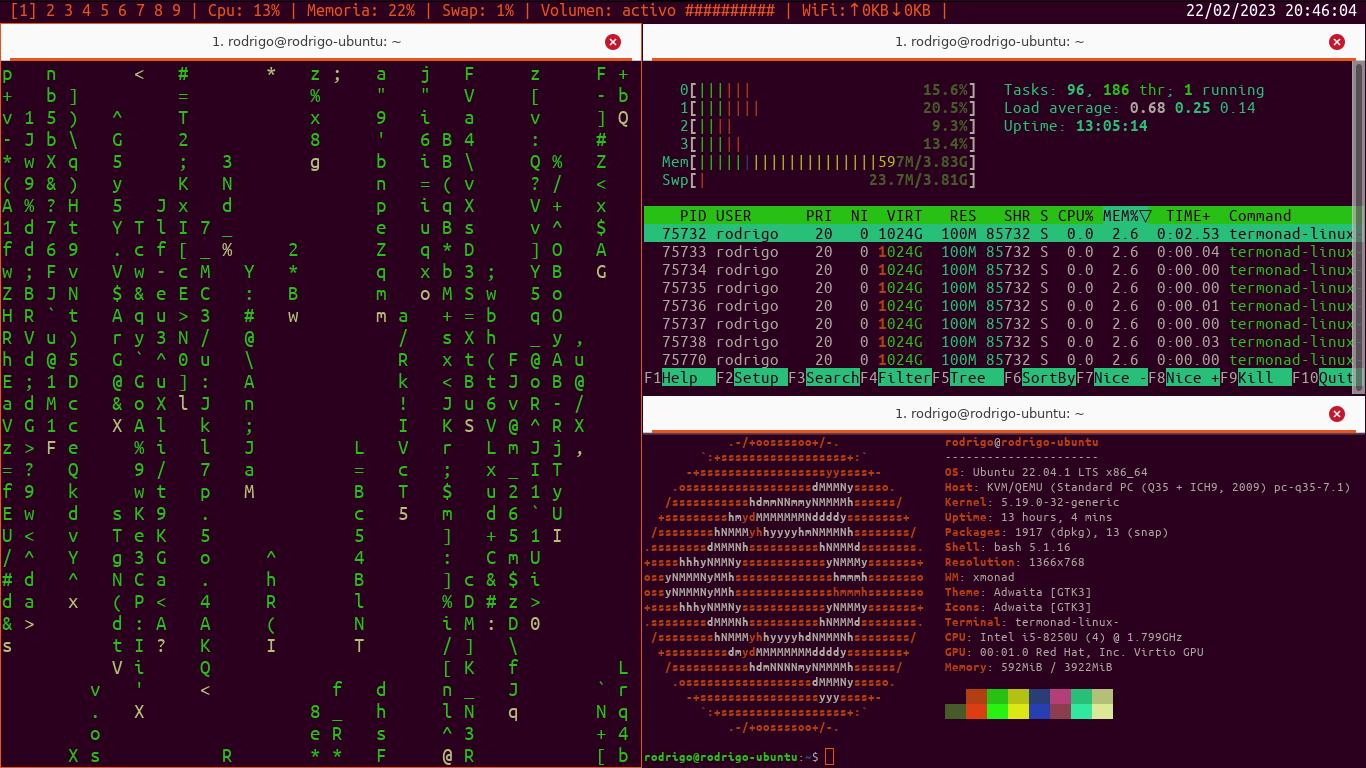
\includegraphics[width=\textwidth]{resultado1}
\end{figure}
\begin{figure}[!ht]
  \caption{Segunda captura de \acrshort{mv}}
  \centering
  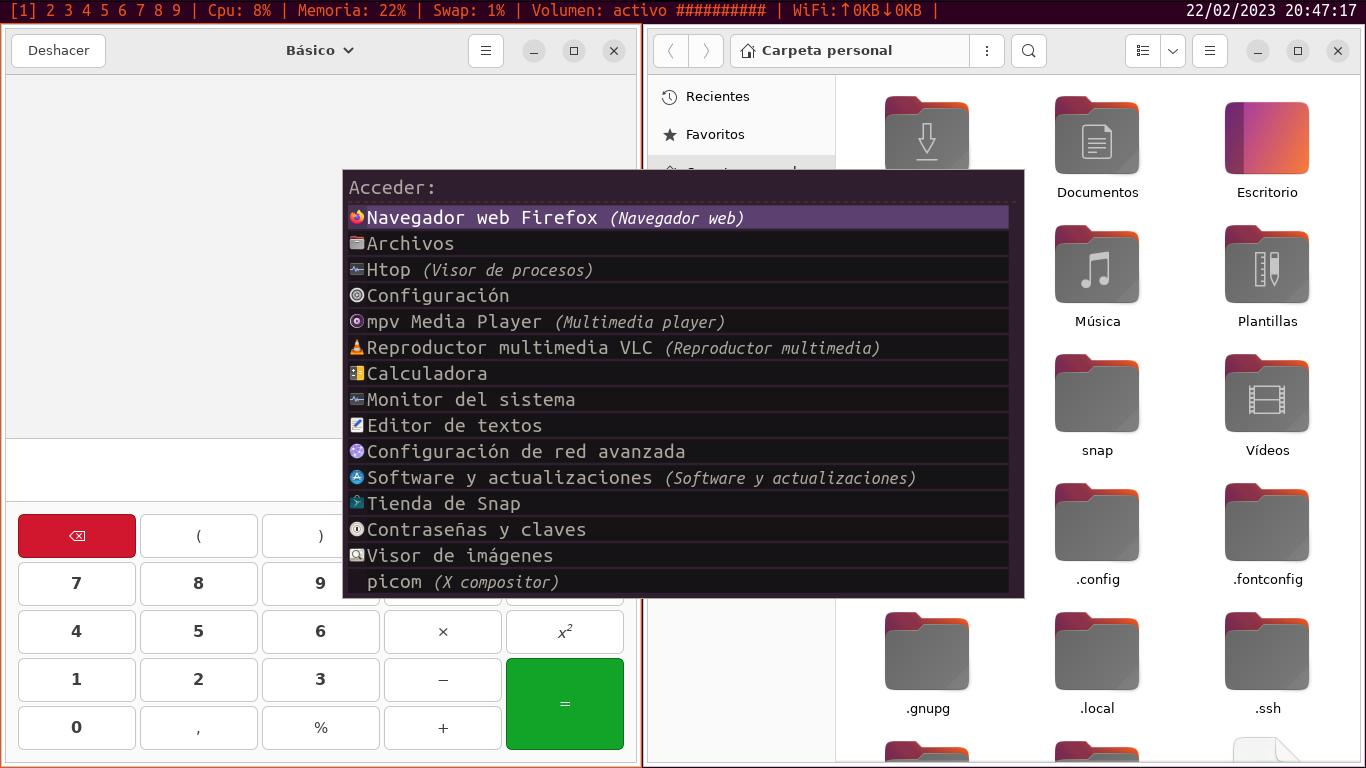
\includegraphics[width=\textwidth]{resultado2}
\end{figure}
\newpage
\begin{figure}[!ht]
  \caption{Tercera captura de \acrshort{mv}}
  \centering
  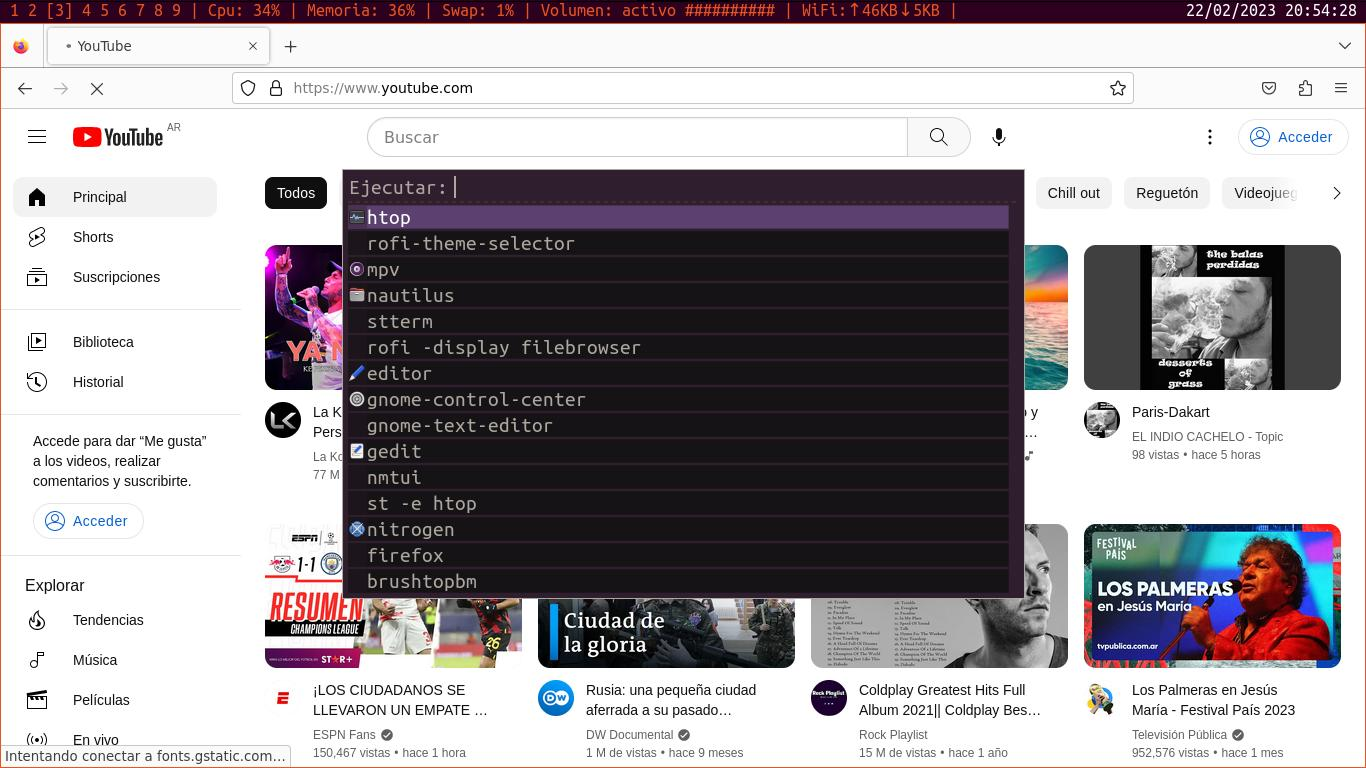
\includegraphics[width=\textwidth]{resultado3}
\end{figure}
\begin{figure}[!ht]
  \caption{Cuarta captura de \acrshort{mv}}
  \centering
  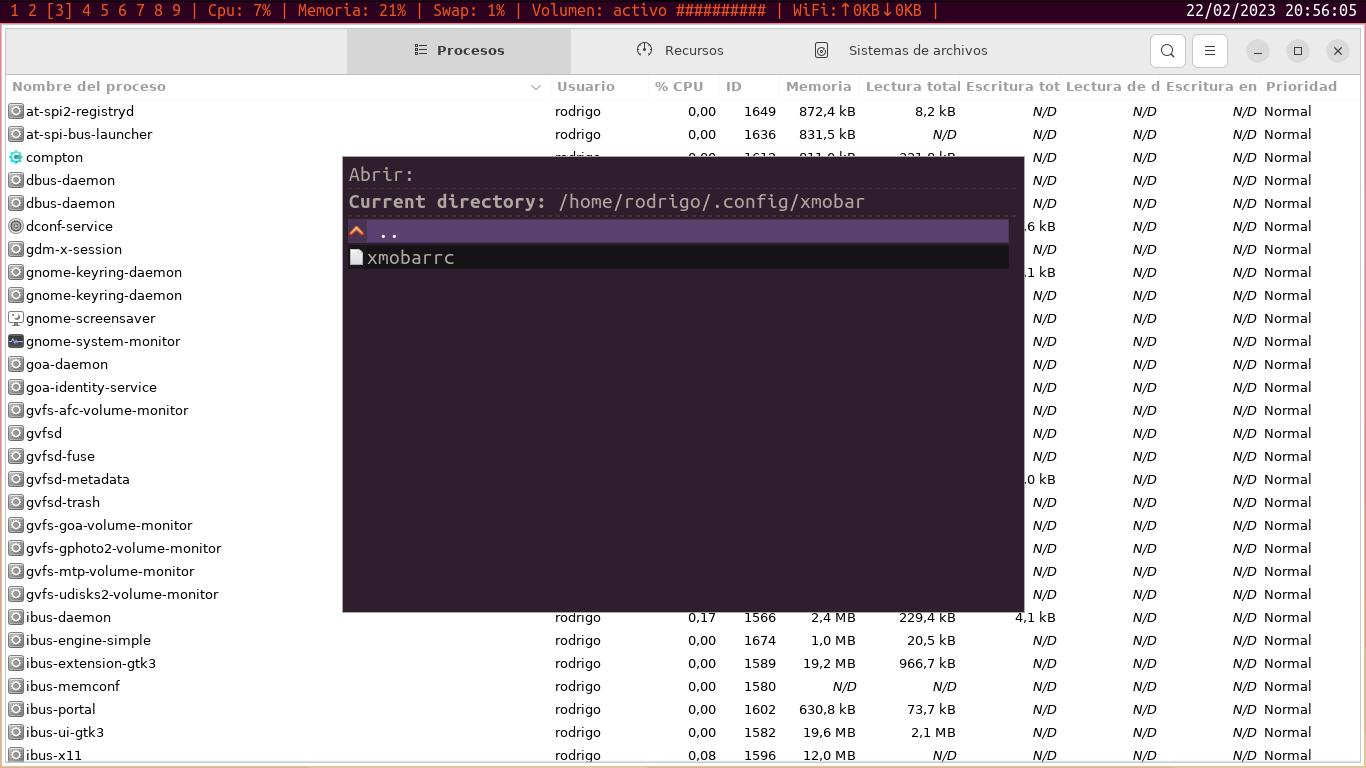
\includegraphics[width=\textwidth]{resultado4}
\end{figure}
\newpage
\begin{figure}[!ht]
  \caption{Quinta captura de \acrshort{mv}}
  \centering
  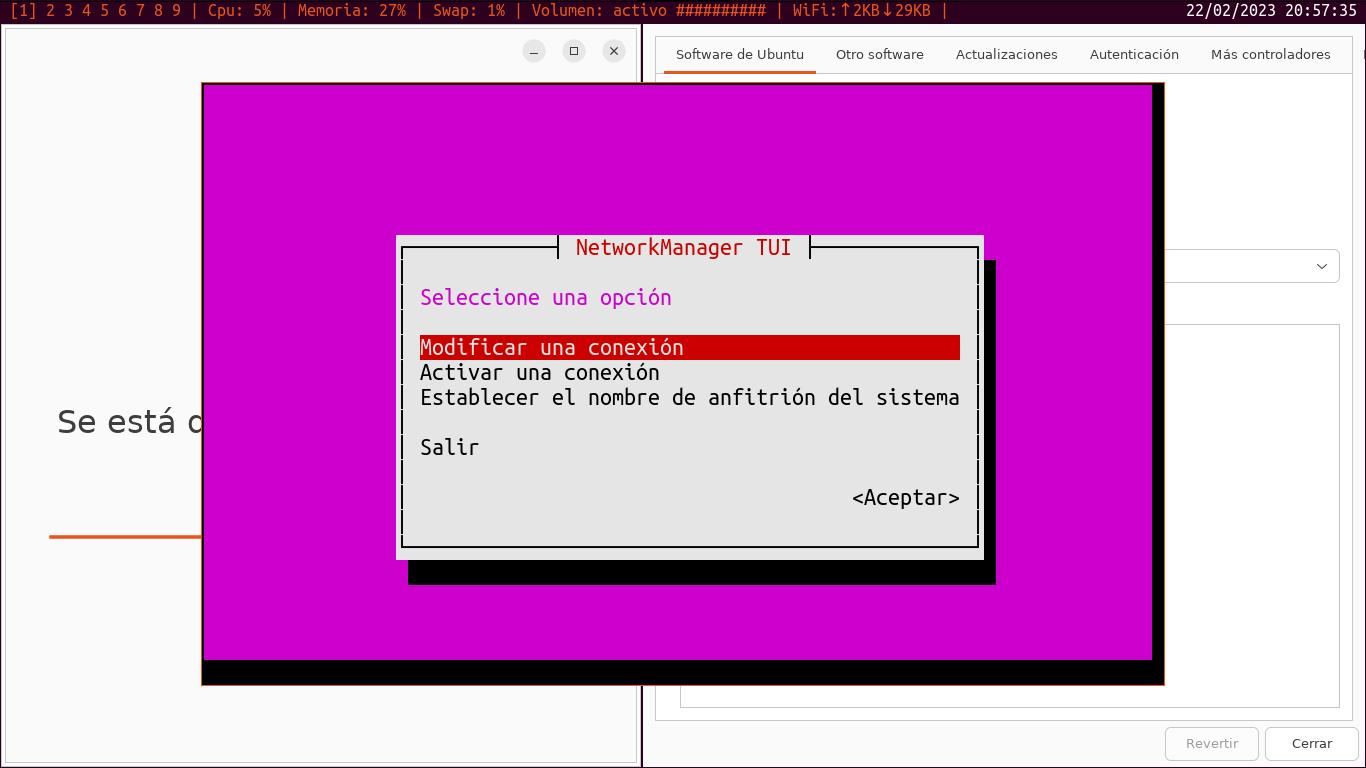
\includegraphics[width=\textwidth]{resultado5}
\end{figure}
\begin{figure}[!ht]
  \caption{Sexta captura de \acrshort{mv}}
  \centering
  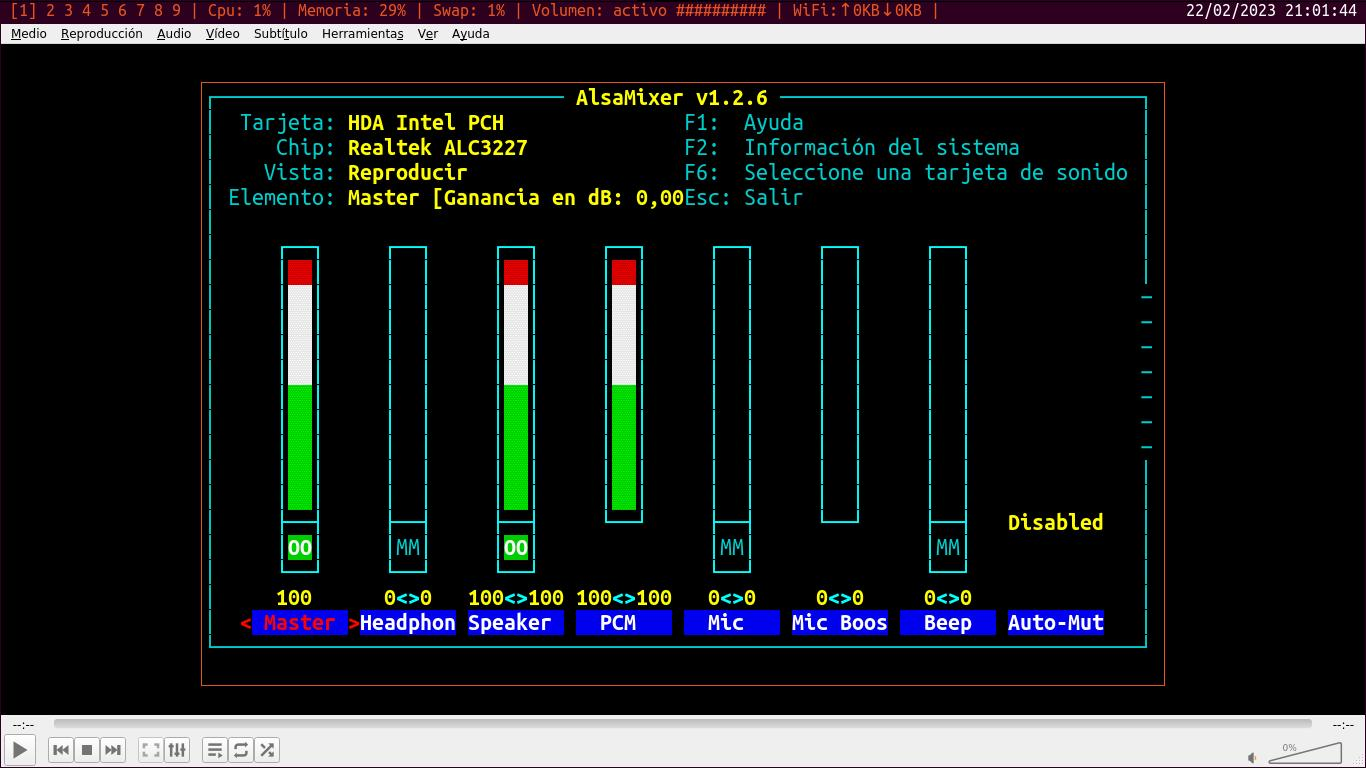
\includegraphics[width=\textwidth]{resultado6}
\end{figure}
\newpage
\begin{figure}[!ht]
  \caption{Séptima captura de \acrshort{mv}}
  \centering
  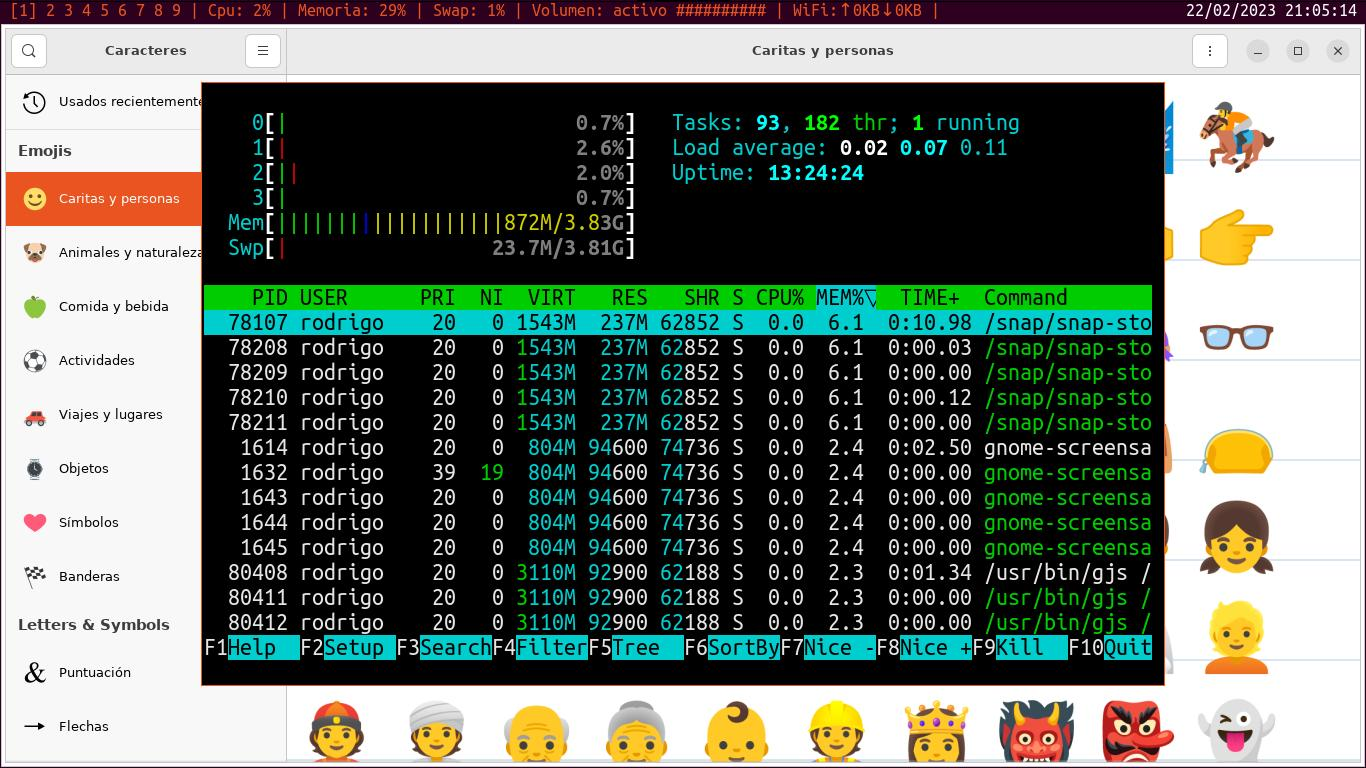
\includegraphics[width=\textwidth]{resultado7}
\end{figure}
\begin{figure}[!ht]
  \caption{Octava captura de \acrshort{mv}}
  \centering
  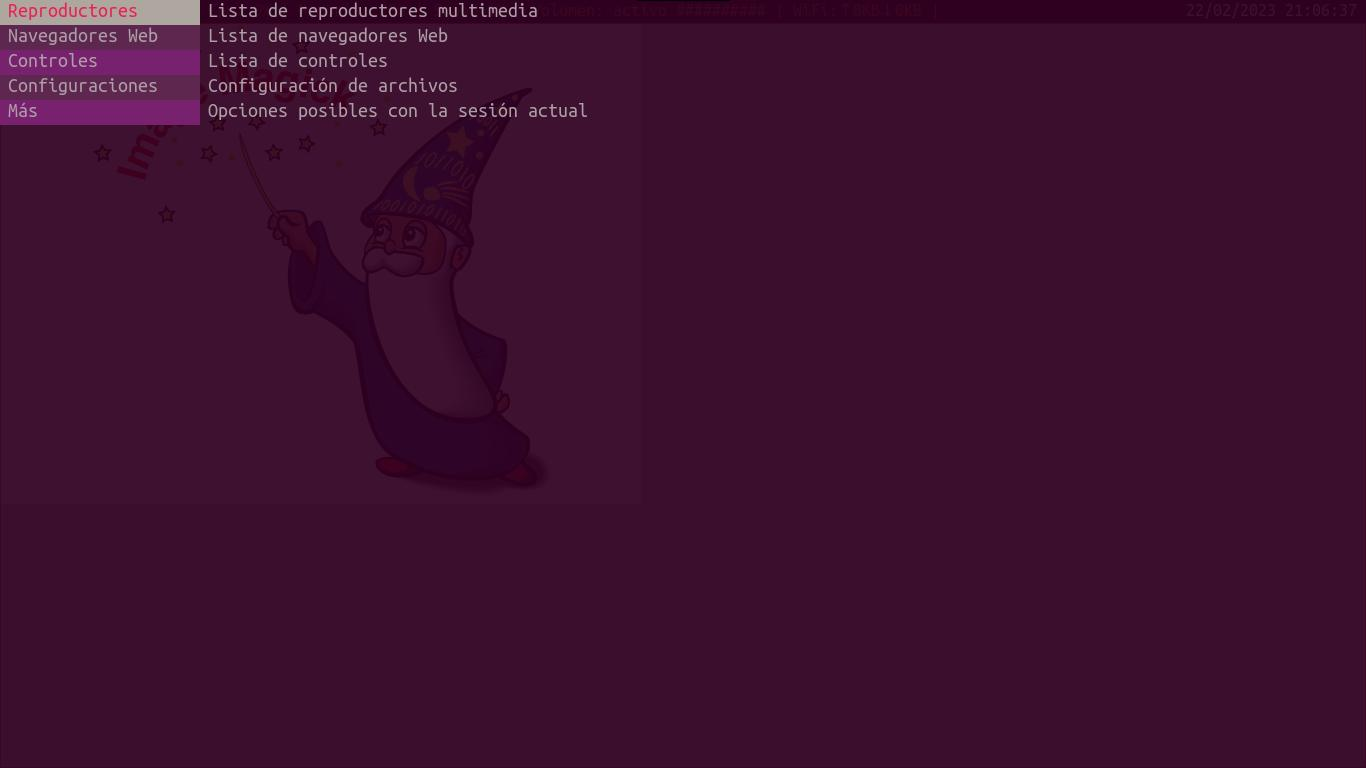
\includegraphics[width=\textwidth]{resultado8}
\end{figure}
\newpage
\begin{figure}[!ht]
  \caption{Novena captura de \acrshort{mv}}
  \centering
  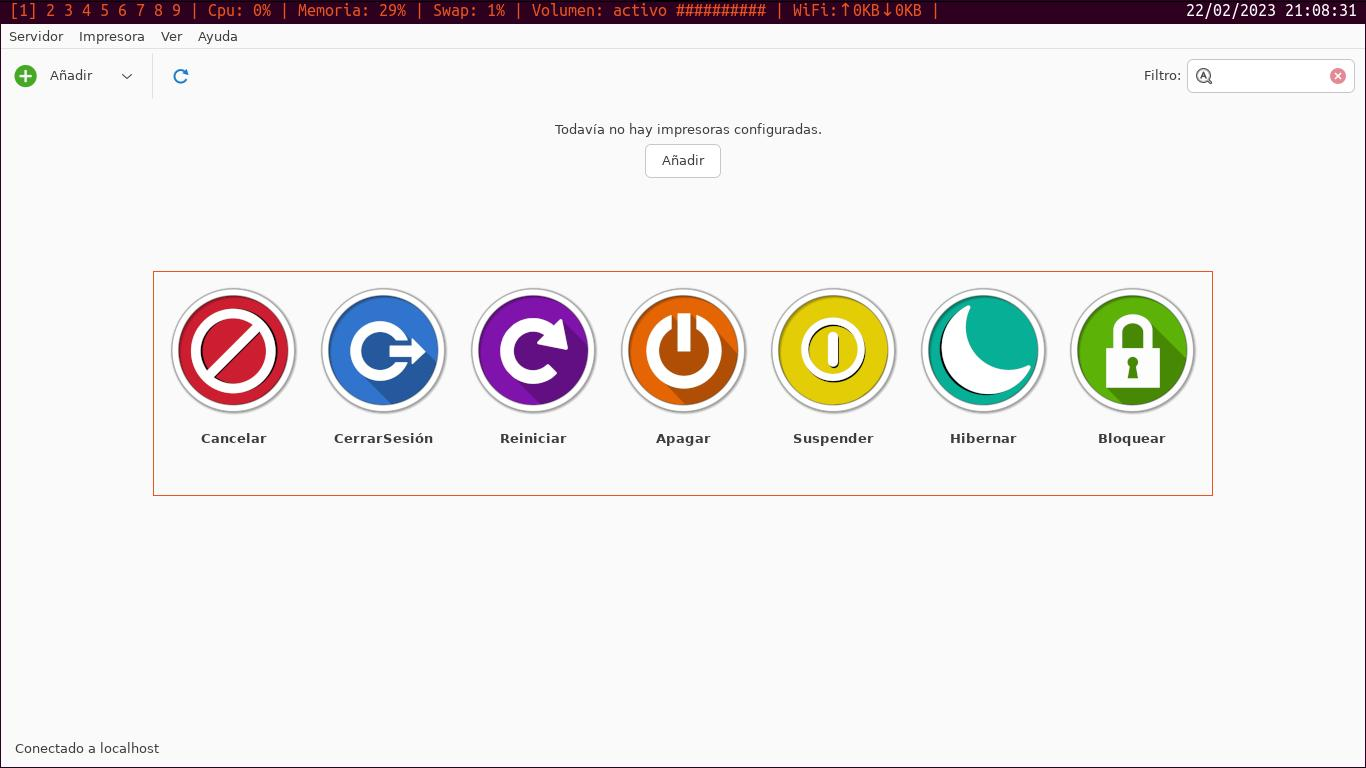
\includegraphics[width=\textwidth]{resultado9}
\end{figure}